%% img/NPClass/HAMTSP.tex
%% Copyright 2019 Andrea Berlingieri
%
% This work may be distributed and/or modified under the
% conditions of the LaTeX Project Public License, either version 1.3
% of this license or (at your option) any later version.
% The latest version of this license is in
%   http://www.latex-project.org/lppl.txt
% and version 1.3 or later is part of all distributions of LaTeX
% version 2005/12/01 or later.
%
% This work has the LPPL maintenance status `maintained'.
%
% The Current Maintainer of this work is Andrea Berlingieri.
%
% This work consists of all files listed in manifest.txt
\documentclass{standalone}

\usepackage{../TikzStyle}
\usepackage{../mystyle}
%\usetikzlibrary{decorating}
\usetikzlibrary{positioning}

\newcommand{\GraphG}[3]{% x,y,name
    \node[point] (#3_m1) at ([shift={(#1 cm,#2 cm)}]0,0) {};
    \node[point] (#3_m2) [right=1cm of #3_m1] {};
    \node[point] (#3_m3) [above right=1cm of #3_m2] {};
    \node[point] (#3_m4) [below right=1cm of #3_m2] {};
    \draw (#3_m1) -- (#3_m2) -- (#3_m3);
    \draw (#3_m2) -- (#3_m4);
}

\begin{document}
    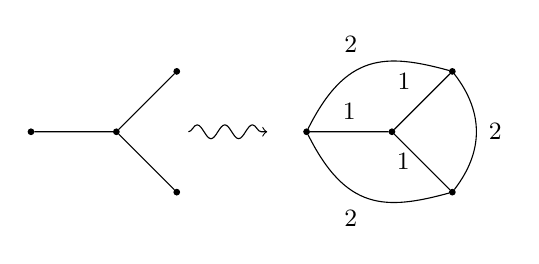
\begin{tikzpicture}[point/.style={draw,circle,inner sep=0cm,fill=black,minimum size=2pt}]
        \GraphG{0}{0}{g1};
        \draw[decorate,decoration=snake,->] (2,0) -- (3,0);
        \GraphG{3.5}{0}{g2};
        \path (g2_m1) -- (g2_m2) node [pos=0.5,above=1pt] {\small 1};
        \path (g2_m2) -- (g2_m3) node [pos=0.5,above left=1pt] {\small 1};
        \path (g2_m2) -- (g2_m4) node [pos=0.5,left=1pt] {\small 1};
        \draw (g2_m1) .. controls (4,1) and (4.5,1) .. (g2_m3) node[pos=0.5,above left=1pt] {\small
        2};
        \draw (g2_m1) .. controls (4,-1) and (4.5,-1) .. (g2_m4) node[pos=0.5,below left=1pt]
        {\small 2};
        \draw (g2_m4) .. controls (5.75,-0.25) and (5.75,0.25) .. (g2_m3) node [pos=0.5,right=1pt]
        {\small 2};
    \end{tikzpicture}
\end{document}
